\chapter{Fonctionnalités}
\label{s:fonctionnalite}

\section{Image}
\subsection{Importation}
Non implémenté

\subsection{Exportation}
L'exportation en image est implémentée grâce à la méthode imageExport de la classe renderer. Tout d’abord, on dessin la scène, sans l’interface graphique. Ensuite, on sauvegarde une capture de l’écran avec le nom, un time stamp, pour que le fichier soit unique, et l’extension reçu en paramètre.

\begin{lstlisting}
void renderer::imageExport(const string name, const string extension)
{
	draw();
	
	ofImage imageTemp;
	
	// extraire des données temporelles formatées
	string timestamp = ofGetTimestampString("-%y%m%d-%H%M%S-%i");
	
	// générer un nom de fichier unique et ordonné
	string fileName = name + timestamp + "." + extension;
	
	// capturer le contenu du framebuffer actif
	imageTemp.grabScreen(0, 0, ofGetWindowWidth(), ofGetWindowHeight());
	
	// sauvegarder le fichier image
	imageTemp.save(fileName);
	
	ofLog() << "<export image: " << fileName << ">";
}
\end{lstlisting}


\subsection{Espace de couleur}
 L'espace de couleur utilisé par l'application est le HSB. Ainsi, pour chaque couleur à saisir, trois «sliders» sont disposer dans l'interface pour saisir la teinte (Hue), la saturation (Saturation) et la valeur (Brightess).
 
 En soit, à chaque mise à jours de l'application, l'application met à jours les valeurs des attributs de couleur dans la classe renderer. Ainsi, à chaque instant, le renderer a les couleurs entrées par l'utilisateur.
 
 Voici un exemple d'initiation des valeurs pour la couleur de remplissage:
 \begin{lstlisting}
 	fillHue.setName("Teinte");
 	fillHue.setMin(0);
 	fillHue.setMax(255);
 	fillHue.set(0);
 
 	fillSaturation.setName("Saturation");
 	fillSaturation.setMin(0);
 	fillSaturation.setMax(255);
 	fillSaturation.set(100);
 
 	fillBrightess.setName("Valeur");
 	fillBrightess.setMin(0);
	fillBrightess.setMax(255);
	fillBrightess.set(255);
 
 	fillAlpha.setName("Transparence");
 	fillAlpha.setMin(0);
 	fillAlpha.setMax(255);
 	fillAlpha.set(255);
 \end{lstlisting} 

Voici la méthode qui génère les couleurs à partir de l'espace HSB:
\begin{lstlisting}
	void ofApp::setColors()
	{
		stroke = ofColor::fromHsb(strokeHue, strokeSaturation, strokeBrightess, strokeAlpha);
		fill = ofColor::fromHsb(fillHue, fillSaturation, fillBrightess, fillAlpha);
		background = ofColor::fromHsb(bgHue, bgSaturation, bgBrightess);
	}
\end{lstlisting} 

Voici la méthode qui met à jours les couleurs du renderer (et l'épaisseur de lignes):
\begin{lstlisting}
	void ofApp::setRendererParameter() {
		
		rend->stroke = stroke;
		rend->fill = fill;
		rend->background = background;
		
		rend->strokeThickness = strokeThickness;
	}
\end{lstlisting}


\subsection{Traitement d'image}
Implémenté

\subsection{Image procédurale}
Non implémenté

\section{Dessin vectoriel}
\subsection{Curseur dynamique}
Implémenté

\subsection{Primitives vectorielles}
Implémenté

\subsection{Formes vectorielles}
Implémenté

\subsection{Outils de dessin}
L'outil de dessin a été implémenté en ajoutant des «sliders» dans l'interface afin de pouvoir modifier la couleur de remplissage, la couleur du contour, la couleur d'arrière plan et l'épaisseur des lignes de contour. Ainsi, il possible de modifier en tout temps la couleur d'arrière plan ou bien de modifier la couleur de remplissage, la couleur de contour et l'épaisseur des lignes de contour pour la création de primitive.

En pratique, à chaque mise à jour de l'application, les valeurs des attributs de la classe renderer sont mises à jour. Ainsi, les valeurs de couleurs ou d'épaisseur des lignes sont à jour lors de la création d'une primitive, tout comme la couleur d'arrière plan est à jour lorsque l'arrière plan est redéssiné.  

Voici la méthode qui met à jours les couleurs et l'épaisseur de lignes du renderer:
\begin{lstlisting}
	void ofApp::setRendererParameter() {
		
		rend->stroke = stroke;
		rend->fill = fill;
		rend->background = background;
		
		rend->strokeThickness = strokeThickness;
	}
\end{lstlisting}

Voici la méthode qui affiche à l'écran le contenu du renderer. La première ligne consiste a déssiner l'arrière plan:
\begin{lstlisting}
	void renderer::draw()
	{
		ofClear(background);
		
		[...]
	}
\end{lstlisting}

Voici une des méthodes qui ajoute une primitive à la scène. Les paramètres «fill» et «stroke» utilisé ici sont les attributs de couleurs de remplissage et de contour de la classe renderer:
\begin{lstlisting}
	ofParameter<bool> renderer::createSquare(float x, float y, float w, float h) {
		return createSquare(x,y,w,h,fill, stroke);
	}
\end{lstlisting}

\subsection{Interface}
L'application est dotée d'une interface utilisateur qui permet de modifier les paramètres d'une primitive à ajouter, ajouter une primitive à la scène, vider la scène, modifier les paramètres de la caméra, appliquer des transformations sur les primitives ou sur la scène, appliquer des effets de traitement d'image, sélectionner des primitives à l'aide d'une liste à cocher, importer un modèle 3D, exporter en image et quitter. 

L'interface a été développé avec «l'addons» ofxGui. Ainsi, nous avons créé des «panels» (ofxPanel) dans lesquels les différents paramètres de l'application ont été ajouté et «l'addons» se chargeait de générer les «sliders» et les cases à cocher associées aux paramètres. Nous avons aussi pu ajouté des boutons (ofxButton).

Comme l'essentiel du code de la classe qui gère l'interface représente plus de 1000 lignes, seulement quelques exemples seront montrés afin d'allégé ce document.

Voici l'initialisation de paramètres:
\begin{lstlisting}
void ofApp::initOfParameters() 
{
	[...]
	
	primPosX.setName("X");
	primPosX.setMin(MinX);
	primPosX.setMax(MaxX);
	primPosX.set((MinX + MaxX) / 2);
	
	primPosY.setName("Y");
	primPosY.setMin(MinY);
	primPosY.setMax(MaxY);
	primPosY.set((MinY + MaxY) / 2);
	
	primPosZ.setName("Z");
	primPosZ.setMin(MinZ);
	primPosZ.setMax(MaxZ);
	primPosZ.set((MinZ + MaxZ) / 2);
	
	[...]
}
\end{lstlisting}

Voici l'initialisation de groupes de paramètres (ofParameterGroup):
\begin{lstlisting}
void ofApp::initGroups()
{
	[...]
	
	groupPrimitivePosition2D.setName("Position");
	groupPrimitivePosition2D.add(primPosX.set(primPosX));
	groupPrimitivePosition2D.add(primPosY.set(primPosY));
	
	groupPrimitivePosition3D.setName("Position");
	groupPrimitivePosition3D.add(primPosX.set(primPosX));
	groupPrimitivePosition3D.add(primPosY.set(primPosY));
	groupPrimitivePosition3D.add(primPosZ.set(primPosZ));
	
	[...]
}
\end{lstlisting}

Voici la configuration de menu:
\begin{lstlisting}
void ofApp::setupMenu2D() {

	menu2D.setDefaultWidth(200);
	
	menu2D.setup();
	
	menu2D.add(groupPrimitiveType2D);
	menu2D.add(groupPrimitivePosition2D);
	menu2D.add(groupPrimitiveSize2D);
	
	menu2D.add(groupThick);
	
	menu2D.add(groupFill);
	
	menu2D.add(groupStroke);
	
	menu2D.add(groupTexture);
	
	menu2D.minimizeAll();
	
	menu2D.registerMouseEvents();
}
\end{lstlisting}

Voici la configuration des écouteurs sur les différents boutons de l'application:
\begin{lstlisting}
void ofApp::initButtonListener() {
	btnDrawPrimitive.addListener(this, &ofApp::btnDrawPrimitiveClicked);
	btnClear.addListener(this, &ofApp::btnClearClicked);
	btnExit.addListener(this, &ofApp::btnExitClicked);
	
	btnExport.addListener(this, &ofApp::btnExportClicked);
	btnImport.addListener(this, &ofApp::btnImportClicked);
	
	btnApplySelect.addListener(this, &ofApp::btnApplySelectClicked);

\end{lstlisting}

Voici la méthode setup de la classe ofApp:
\begin{lstlisting}
void ofApp::setup()
{
	[...]
	
	initOfParameters();
	initGroups();
	
	setupMenu2D();
	setupMenu3D();
	setupCameraMenu();
	setupTransformationMenu();
	setupOptionMenu();
	setupSelectionMenu();
	
	initButtonListener();
	
	[...]
}
\end{lstlisting}

Voici une capture d'écran pour montré l'interface:
\begin{figure}[h]
	\centering
	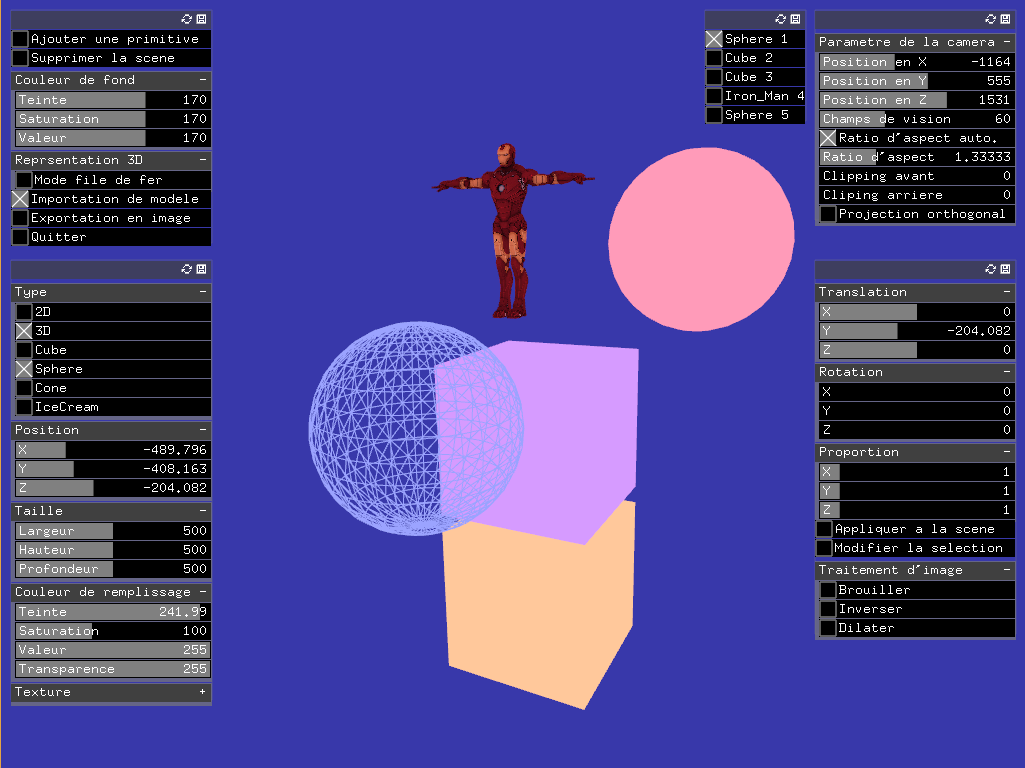
\includegraphics[width=15cm]{fig/InterfaceComplet.png}
	\caption{Exemple d'interface}
	\label{fig:interface}
\end{figure}

\section{Transformation}
\subsection{Transformation interactive}
Implémenté

\subsection{Structure de scène}
La structure de scène a été implémenté sous la forme d'un arbre ordoné, dans lequel les feuilles sont les éléments de la scène. La classe scène comprend 4 classes interne, soit element, group, node et scene\_iterator. Les classes group et node héritent d'element et  servent à stocker tout ce qui se trouve dans la scène. La classe scene\_iterator permet, quant-à elle, de parcourir les éléments pour les dessiner. 

On utilise les shared\_ptr au lieux des simples pointeurs pour conserver les éléments qui sont ajouté à la scène pour ne pas avoir à trop gérer la mémoire.

L'essentiel du code de la scène se trouve dans les méthodes addElement de la scène, des sous-clases de stockage et l'operator++ de l'itérateur.

\begin{lstlisting}
void scene::addElement(size_t index, primitive_ptr& p, bool insertFirstChild) {
	if (index == 0 && !insertFirstChild {
		throw invalid_argument("root don't have parent...");
	}
	root->addElement(index, p, insertFirstChild);
}

//Retourne la quantite d'element ajoute
size_t scene::node::addElement(size_t index, primitive_ptr& p, bool insertFirstChild) {
	if (index != this->index) {
		throw invalid_argument("index need to be equals to the index of the node");
	}
	if (insertFirstChild) {
		throw invalid_argument("node need to be wraped in a group");
	}
	this->content = p;
	contentType = "primitive";
	return 1;
}

//Retourne la quantite d'element ajoute
size_t scene::group::addElement(size_t index, primitive_ptr& p, bool insertFirstChild) {
	size_t addedSize = 0;
	
	if (this->index == index) {
		if (insertFirstChild) {
			//Inserer comme premier element
			childrens.insert(childrens.begin(), element_ptr{ new node{ index + 1, height + 1, p } });
			for (auto& it = childrens.begin() + 1; it < childrens.end(); ++it) {
				it->get()->setIndex(it->get()->getIndex() + 1);
			}
			addedSize++;
		} else {
			throw invalid_argument("element must to be add in the parent");
		}
	} else {
		size_t ubound = childrens.size();
		size_t lbound = 0;
		size_t i;
		
		//Recherche binaire
		while (lbound <= ubound) {
			i = lbound + (ubound - lbound) / 2;
			if (childrens[i]->getIndex() == index) {
				if (insertFirstChild) {
					if (childrens[i]->getType() != "group") {
						group_ptr temp = group_ptr{ new group{ index, height + 1 } };
						temp->childrens.push_back(childrens[i]);
						temp->childrens[0]->setIndex(index + 1);
						temp->childrens[0]->setHeight(height + 2);
						temp->size = temp->childrens[0]->getSize() + 1;
						childrens[i] = temp;
						addedSize++;
					}
					addedSize += childrens[i]->addElement(index, p, insertFirstChild);
				} else {
					childrens.insert(childrens.begin() + i + 1, element_ptr{ new node{ index + childrens[i]->getSize(), height + 1, p } });
					i++;
					addedSize++;
				}
				i++;
				break;
			} else if (childrens[i]->getIndex() < index) {
				lbound = i + 1;
				if (ubound < lbound) {
					//Ajoute l'element dans le groupe sous-jacent
					addedSize += childrens[i]->addElement(index, p, insertFirstChild);
					i++;
					break;
				}
			} else {
				ubound = i - 1;
				if (ubound < lbound) {
					//Ajoute l'element dans le groupe sous-jacent
					addedSize += childrens[i - 1]->addElement(index, p, insertFirstChild);
					break;
				}
			}
		}	
		for (auto& it = childrens.begin() + i; it < childrens.end(); ++it) {
			it->get()->setIndex(it->get()->getIndex() + addedSize);
		}
	}
	size += addedSize;
	return addedSize;
}

//Avance jusqu'au prochain node
void scene::scene_iterator::operator++() {
	for (rootIndex; rootIndex <= root->getSize(); ++rootIndex) {
		element* elem = root->getElement(rootIndex);
		if (elem->getType() != "group" && elem->getType() != "root") {
			primitive_ptr ptr = (dynamic_cast<node*>(elem))->content;
			if (p != ptr) {
				p = ptr;
				break;
			}
		}
	}
	if (rootIndex > root->getSize()) {
		p = primitive_ptr{ nullptr };
	}
}
\end{lstlisting}
Comme vous avez sans-doute remarqué, l'ajout d'élément à la scène se fait récursivement, à l'index en paramètre. Le paramètre «insertFirstChild» indique s'il faut insérer l'élément comme le premier enfant de l'élément à l'index en paramètre. S'il est faux, on insère simplement le nouvel élément après l'index. Dans group::addElement, on utilise un algorithme de recherche binaire pour trouver dans ou après quel élément il faut ajouter le nouvel élément.

L'operator++, quant à lui, parcours la scène en s'arrêtant seulement sur les classes node.  

Malheureusement, par manque de temps la structure de scène n'est pas utilisé à sont plein potentiel et tous les éléments sont stocké dans le groupe à la racine de la scène. Il est tout de même possible de voir le résultat en changeant la ligne «\#define test 0» pour «\#define test 1» dans le fichier «main.cpp». Vous verrez alors le résultat de l'exécution des tests de la classe scene (principalement de l'ajout et de la supression d'élément), se trouvant à la fin de «scene.cpp». 

\subsection{Sélection multiple}
Implémenté

\subsection{Coordonnées non-cartésiennes}
Non-implémenté

\subsection{Historique}
Non-implémenté

\section{Géométrie}
\subsection{Particules}
Non-implémenté

\subsection{Primitives}
Implémenté

\subsection{Modèle}
Implémenté

\subsection{Texture}
Implémenté

\subsection{Géométrie procédurale}
Non-implémenté

\pagebreak
\section{Caméra}
\subsection{Propriétés de caméra}
Helllo there????

\begin{figure}[h]
	\centering
	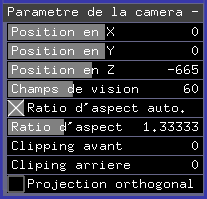
\includegraphics[width=5cm]{fig/proprieteCamera.png}
	\caption{Propriété de la caméra dans l'interface}
	\label{fig:test}
\end{figure}

\subsection{Mode de projection}
Le changement de mode de projection de perspective à orthogonale a été implémenté dans l'application. L'essentiel du travail se fait dans la méthode ccamera::changeMode(). Elle est appelé lorsqu'on appuit sur le bouton à cet effet dans l'interface graphique.

\begin{lstlisting}
	if (ortho.get()) {
		cam->enableOrtho();
	} else {
		cam->disableOrtho();
	}
\end{lstlisting}

\subsection{Caméra interactive}
La caméra interactive est implémenter dans l'application principalement à l'aide de la classe ofEasyCam de openFrameworks. Nous avons tout de même ajouter la possibilité de déplacer à l'aide des flèches du clavier, pour permettre de repositionner facilement la caméra. Il est aussi possible d'avancer à caméra à l'aide de pageUp/Down. L'essentiel du code se trouve au début de «ccamera::update()».

\begin{lstlisting}
	float dist = speed * dt;
	float dx = 0;
	float dy = 0;
	float dz = 0;
	
	dx = 0;
	if (isCameraMoveLeft)
		dx += dist;
	if (isCameraMoveRight)
		dx -= dist;
	cam->truck(-dx);
	posX.set(round(-cam->getX()));
	
	dy = 0;
	if (isCameraMoveUp)
		dy -= dist;
	if (isCameraMoveDown)
		dy += dist;
	cam->boom(-dy);
	posY.set(round(cam->getY()));
	
	dz = 0;
	if (isCameraMoveForward)
		dz -= dist;
	if (isCameraMoveBackward)
		dz += dist;
	cam->dolly(dz);
	posZ.set(round(cam->getZ()));
\end{lstlisting}

\subsection{Caméra multiple}
Non-implémenté

\subsection{Caméra animée}
Non-implémenté
